\documentclass[12pt]{article}

\usepackage{amsmath}
\usepackage{float}
\usepackage[margin=1.2in]{geometry}
\usepackage{listings}
\usepackage{color}
\usepackage{graphicx}
\usepackage{caption}
\usepackage{newfloat}
\usepackage{subcaption}
\usepackage{amssymb}

\bibliography{ref}

\DeclareCaptionType{snip}[Typename][List of snippet]
\newenvironment{snippet}{\captionsetup{type=snippet}}{}


\DeclareFloatingEnvironment{Snippet}
\title{\bfseries Sorting Algorithms}
\author{Benjamin Hough, Erick Sanchez}
\date{May 18, 2016}

\usepackage{array}
\setlength\extrarowheight{2pt} 


\lstset{
	language=[Visual]C++,
	basicstyle=\footnotesize, 
	keywordstyle=\bfseries\ttfamily\color[rgb]{0,0,1},
	identifierstyle=\ttfamily,
	commentstyle=\color[rgb]{0.133,0.545,0.133},
	stringstyle=\ttfamily\color[rgb]{0.627,0.126,0.941},
	showstringspaces=false,
	numberstyle=\footnotesize,
	numbers=left,
	stepnumber=1,
	numbersep=10pt,
	tabsize=2,
	breaklines=true,
	prebreak = \raisebox{0ex}[0ex][0ex]{\ensuremath{\hookleftarrow}},
	breakatwhitespace=false,
	aboveskip={1.5\baselineskip},
	columns=fixed,
	extendedchars=true
	% frame=single,
	% backgroundcolor=\color{lbcolor},
}


\begin{document}
	
	\maketitle
	
	\section*{Abstract}
	
	The abstract will go here and will look awesome when it renders
	
	\tableofcontents
	
	\pagebreak
	
	
	
	\section{Introduction} %"Introduction - Give a short but informative introduction to your chosen topic, including the current “state of the field” as appropriate. Outline what you will do in the balance of the paper (ie. Explain the goals of the paper). Indicate why this topic is exciting/useful."
	
	 Sorting algorithms are a fundamental type of algorithms that many other more sophisticated algorithms are built upon.
	 In the most abstract form sorting algorithms take in a list of unordered items and output or modify the list to the desired order, whatever it may be (typically numeric or alphabetic order is used).
	 The goal of our research was to gain a better understanding of sorting algorithms in general  and to learn the nuances between the different types of algorithms available. 
	 We wanted to learn what a makes a sorting algorithm efficient what are the limitations of the efficiency. 
	 This paper will go over definitions associated with sorting algorithms and it will cover the two broad categories of sorting algorithms, comparison and non-comparison. 
	 Next it will examine sorting efficiencies, different applications of sorting algorithms, and methods for choosing the appropriate algorithm for a given application. 
	 It is assumed that the reader has a basic understanding of what an algorithm is and has been exposed to pseudocode in some form. 
	
	\section{Background} %"Introduce any new definitions, notation, or other background information necessary for understanding the rest of the paper. (Your audience is your classmates in Math 4, not your professor.) Depending on your subject, your background and introduction sections might be combined."
	
	Since there is coding and syntax involved, only 
	``\underline{input} sequence is called an instance of the sorting problem"\cite[p.~5]{intro}\newline
	``An algorithm is said to be \underline{correct} if, for every input instance, it halts with the correct output. We say that a correct algorithm \underline{solves} the given computational problem"(Introduction to Algorithms)\cite[p.~6]{intro}\newline
	``The number that we wish to be sort are also known as the \underline{keys}"(Introduction to Algorithms)\cite[p.~16]{intro}\newline
	``An \underline{algorithm} is a procedure or formula for solving a problem."\cite{wiki}\newline
	``A \underline{compiler} is a computer program ... that transforms source code written in a programming language ... into another computer language …, with the latter often having a binary form known as object code."\cite{wiki}\newline
	``The \underline{call stack} is a stack data structure that stores information about the active subroutines of a computer program"\cite{wiki} Whenever a function calls a new function, this adds to the stack.\newline
	``A \underline{recursion function} (DEF) is a function which either calls itself"\cite{wiki} When a function calls itself, there needs to be a condition for the function to stop itself; end the recursion. This is called \underline{end case}. The end case does not contain a function call to itself thus stopping the recursion.\newline
	
	\section{Body}
	
	\subsection{Comparison Sorts}
	\label{CompSort}
	Comparison sorts are any sorting algorithms that use logical comparisons to determine element order, typically $>$, $<$, $\ge$, or $\le$ is used.
	quicksort, heap, insertion, selection, merge, etc.
	
	insert insertion sort description
	
	What are they
	How do they work
	When and when not to use them
	
	\begin{center}
	\begin{table}[h]
		\centering
		\begin{tabular}{|l|l|l|l|}
			\hline
			\textbf{Name}  & \textbf{Average}    & \textbf{Worst}      & \textbf{Memory} \\ \hline
			Quicksort      & $ n \cdot log (n) $ & $ n^2 $             & $ log (n) $     \\ \hline
			Merge Sort     & $ n \cdot log (n) $ & $ n \cdot log (n) $ & $ n $              \\ \hline
			Heapsort       & $ n \cdot log (n) $ & $ n \cdot log (n) $ & $ 1 $              \\ \hline
			Insertion Sort & $ n^2 $             & $ n^2 $             & $ 1 $              \\ \hline
			Introsort      & $ n \cdot log (n)$  & $ n \cdot log (n)$  & $ log (n) $     \\ \hline
			Selection Sort & $ n^2 $             & $ n^2 $             & $ 1 $              \\ \hline
			Bubble Sort    & $ n^2 $             & $ n^2 $             & $ 1 $              \\ \hline
		\end{tabular}
		\caption[Comparison Sorting Algorithms]{Common comparison sorting algorithms. $n$ is the number of items being sorted}
		\label{tab:comp}
	\end{table}
\end{center} %rad table file
	
	
	\begin{Snippet}[h]
		\caption[Insertion Sort]{Insertion Sort implementation in C++}	
		\lstinputlisting{InsertionSort.cpp}
		\label{snip:ins}
	\end{Snippet}
	
	
	
	\subsection{Non-Comparison Sorts}
	
	Non-comparison sorts, like the name implies do not rely on the comparison operators $<$,$>$,$\le$,$\ge$ to sort.
	This gives non-comparison sorts a huge speed boost but of course there is a trade off to the increased speed. 
	Unlike the comparison sorts described in \ref{CompSort} which can sort any data that has a defined numerical value, non-comparison sorts rely on certain assumptions about what is being sorted in order to function.
	This sets certain restrictions on the type of data that non-comparison sorts can manage.
	Common non-comparisons sorts include: Radix sort, Burstsort, Postman sort, Bucket sort, and Counting sort.
	We will look at examples of the latter two, Bucket sort and Counting sort  in order to gain an understanding of what makes non-comparison sorts different.

	\begin{center}
	\begin{table}[h]
		\centering
		\begin{tabular}{|l|l|l|l|}
			\hline
			\textbf{Name}   & \textbf{Average} & \textbf{Worst}  & \textbf{Memory} \\ \hline
			Radix sort      & $ n \cdot k/d $  & $ n \cdot k/d $ & $ n+2^d $       \\ \hline
			Burstsort       & $ n \cdot k/d $  & $ n \cdot k/d $ & $ n \cdot k/d $ \\ \hline
			Counting Sort   & $ n+r $          & $ n+r $         & $ n+r $         \\ \hline
			Pigeonhole sort & $ n+2^k $        & $ n+2^k $       & $ 2^k $         \\ \hline
			Postman sort    & $ n \cdot k/d $  & $ n \cdot k/d $ & $ n+2^d $       \\ \hline
		\end{tabular}
		\caption[Non-comparison Sorting Algorithms]{Common non-comparison sorting algorithms. $n$ is the number of elements being sorted, $d$ is the number of digits,  $r$ is the range of values, and $k$ is the key size.}
		\label{tab:noncomp}
	\end{table}
\end{center} %rad table file
	
	\subsection{Efficiency and Memory}
	
	Solving the same sorting problem often comes with the better algorithm when talking about efficiency.
	Computer hardware and software play the biggest role when dealing with efficiency.
	
	\paragraph{Insertion and Merge Sort}
	
	Let’s write insertion sort as $c_1 \cdot\,n^2$ and merge sort as $c_2 \cdot\,n\,\log_2{n}$, $c_1$ and $c_2$ are based off of how efficient the software and compiler are.
	We see that insertion sort has a factor of n, while merge sort has a factor of $\log_2{n}$ which is far smaller.
	But after writing the perfect code, $c_1$ and $c_2$ become closer to 1, getting the best efficiency will have to depend on the hardware and size of the list that needs to be sorted.
	Let’s take a deeper look. Running these two algorithms, insertion sort and merge sort, on two different machines; A and B. Each machine is sorting an array of ten million numbers.
	Machine A executes ten billion instructions per second and machine B executes only ten million per second.
	Thus, machine A is a thousand times faster than machine B.
	The algorithm on machine A is written in machine language that requires 2 $\cdot\;n^2$ instructions to sort n numbers, with $c_1$ = 2.
	For machine B, the algorithm is written using a high-level language with an inefficient compiler that requires 50 $\cdot\;n\;\log_2{n}$ instructions to sort n numbers. $c_2$ = 50, which is a poor constant.
	Machine A takes
	
	$$\frac{2\,\cdot\,(10^7)^2 \;instructions}{10^{10} \;instructions/\!second}=20000\mbox{ seconds ( more than 5.5 hours)}$$
	
	And machine B
	
	$$\frac{50\,\cdot\,10^7\,\log_2{10^7}\;instructions}{10^{7} \;instructions/\!second}\approx1163\mbox{ seconds ( less than 20 minutes)}$$
	                                                                                 
	Looking at this one case, having one algorithm isn't going to be the better one for all cases. Hardware, software, the size of the list, and computer power all add to how efficient a sorting algorithm will be. Why? That's when we need to side 
	                                                                                 
	\subsubsection{Big O Notation}
	
	An algorithm can take at most seconds to finish executing.
	Some can take hours or even years to finish.
	Measuring resources used for an algorithm to execute, the Big O notation would give you the answer.
	But before we understand Big O notation, we’ll look into analyzing insertion sort.
	
	\paragraph{Analysis of Insertion Sort}
	
	The notations we use to describe the asymptotic running time of an algorithm are defined in terms of functions whose domains are the set of natural numbers, $\mathbb{N}$ \{ 1, 2 , 3 .. \}~\cite[p.~43]{intro}
	This is called asymptotic notation.
	For insertion sort, the worst-case is $n^2$ depending on the input of how unsorted the list is.
	The larger the list, the longer it'll take. Thus, we need to define a few things to characterize insertion sort; running time and size of input.
	In some cases, the $\textit{\textbf{input size}}$ can go stretch from number of items in a list to number of bits after adding two number. 
	For insertion sort, it’s going to be the number of elements to be sorted.
	This does not depend on how unsorted the arrangement of number, just the size.
	The $\textit{\textbf{running time}}$ is going to be the number of steps, or instructions.
	Now, each line of code can't always take the same amount of $\textit{time}$ to execute.
	An assignment will take a different amount of $\textit{time}$ than an $\textit{if-else}$ statement.
	
	To better understand, we’ll look at an example for a simple loop.
	Each line of code will take $c_i$ long to execute; $i$ is denoted for each line of code.
	
	\begin{center}
	\begin{table}[h]
		\centering
		\begin{tabular}{lllll}
			& & cost & times                     &  \\
			1 & for j = 1 to n            & $c_1$ & n                     &  \\
			2 & r = 5  & $c_2$ & n                     &  \\
			3 & while ( r \textgreater\;0) & $c_3$ & $\sum_{r=1}^{5}\;t_j$ &  \\
			4 & r -= 1                    & $c_4$ & $\sum_{r=1}^{5}\;t_j$ & 
		\end{tabular}
		\caption{A nested loop, looping n times}
		\label{tab:simpleCode}
	\end{table}
\end{center}
	
	Thus, the $\textit{time}$ it takes to execute this loop is
	\begin{center}
		T(n) = $c_1n$ + $c_2n$ + $c_3\sum_{r=1}^{5}$ + $c_4\sum_{r=1}^{5}$
	\end{center}
	is the characteristic formula for this algorithm shown in Table~\ref{tab:simpleCode}.
	For this linear function it has a factor of $n$ that can be factored to T(n) = ($c_1$ + $c_2$)n + ($c_3$ + $c_4$)$\sum_{r=1}^{5}$, or T(n) = an + b.
	
	Coming back to insertion sort, the characteristic for the best case of insertion sort is
	\begin{center}
		T(n) = ($c_1$ + $c_2$ + $c_4$ + $c_5$ + $c_8$)n - ($c_2$ + $c_4$ + $c_5$ + $c_8$)
	\end{center}
	which can be expressed as an + b for constants a and b that depend on the statement costs $c_i$ as shown below
	
	\begin{center}
	\begin{table}[h]
		\centering
		\begin{tabular}{|l|l|l|l|}
			 \hline
			& & cost & times                      \\ \hline
			1 & for j = 2 to A.length & $c_1$ & n \\ \hline
			2 & key = A[j] & $c_2$ & n - 1 \\ \hline
			3 & ... & $0$ & n - 1 \\ \hline
			4 & i = j - 1                    & $c_4$ & n - 1 \\ \hline
			5 & while i $\textgreater$ 0 and A[i] $\textgreater$ key & $c_5$ &  $\sum_{j=2}^{n}\;t_j$ \\ \hline
			6 & A[i + 1] = A[i] & $c_6$ &  $\sum_{j=2}^{n}\;(t_j\;-\;1)$ \\ \hline
			7 & i = i - 1 & $c_7$ &  $\sum_{j=2}^{n}\;(t_j\;-\;1)$ \\ \hline
		\end{tabular}
		\caption{A nested loop, looping n times}
		\label{tab:insertionCode}
	\end{table}
\end{center}
	
	\paragraph{What is Big O Notation}
	
	def 
	
	\subsection{Exploration of a New Sorting Algorithm}
	
	
	To fulfill the requirement of demonstrating original thought we looked at creating our own sorting algorithm.
	 It proved difficult to come with a new sorting idea with so many existing sorting algorithm already on our mind.
	So instead we took an already well known algorithm and put a twist on it. 
	The standard implementation of Mergesort uses a recursive flow; each iteration calls the sort on itself and splits the list in two until it is completely divided. 
	It then pieces it back together as it sorts. 
	A visual representation of this is shown below.
	
	
\begin{figure}[H]
	
	\begin{subfigure}{0.5\textwidth}
		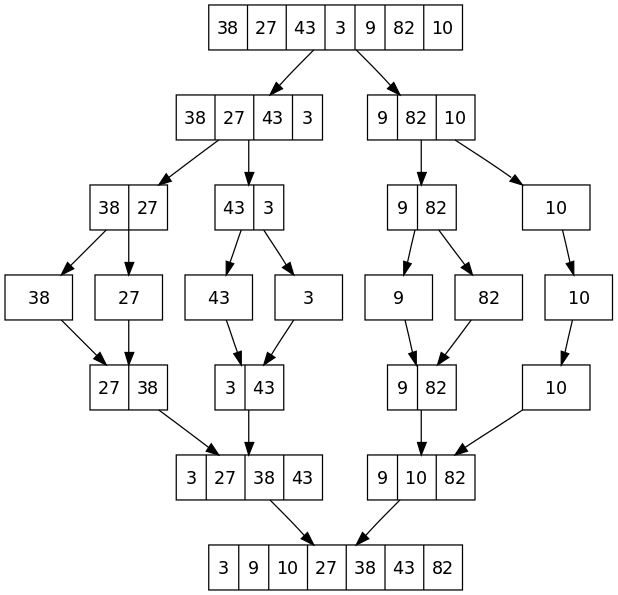
\includegraphics[width=2.5in]{Merge_sort_algorithm_diagram.png} 
		\caption{Standard Mergesort}
		\label{fig:stdmerge}
	\end{subfigure}
	\begin{subfigure}{0.5\textwidth}
		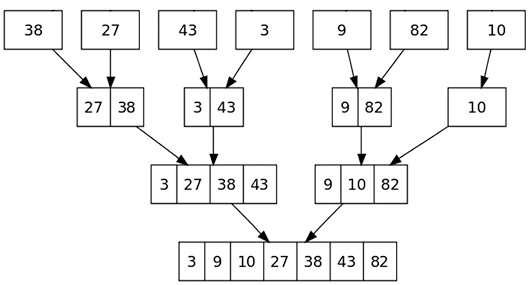
\includegraphics[width=2.5in]{New_merge_sort_algorithm_diagram.png}
		\caption{Our Mergesort}
		\label{fig:newmerge}
	\end{subfigure}
	
	\caption{Algorithm flow of the standard mergesort and our own implementation}
	\label{fig:bothmerge}
\end{figure}
	
	Now onto our variant. 
	We decided to forgo the recursion and keep everything to one function call. 
	The reasoning for this is that recursive functions have an overhead associated with them caused by the increased call stack (local variables must be reinitialized at each level and the entrance of each function call must be stored so it can be returned to when the function exits). 
	By skipping the recursion step it allows the algorithm to start immediately comparing pairs of elements. 
	Visually it is represented by the bottom half of the picture above. 
	The algorithm in its entirety is shown below, it is written in C++.
	
	\begin{center}
		\captionof{Snippet}[New Mergesort]{Our own mergesort implementation that doesn't use recursion. Written in C++}
		\lstinputlisting{mergeSort2.cpp}
		\label{snip:newmerge}
	\end{center}

	Just knowing that an algorithm works is not enough; an analysis of the runtime is also needed to ensure the algorithm performs as needed. 
	The new mergesort algorithm was compared to a standard implementation of mergesort, introsort, quicksort, and insertion sort. 
	To perform the tests, each algorithm was given the same randomly generated list starting with a size of 3 and doubling each time up to 12,582,912 elements. 
	To our surpriswe the new mergesort outperformed many of the other algorithms. 
	As shown in Figure~\ref{fig:algeff}, for lists with over 100 elements and up to the test limit the new mergesort performed 13X faster than the built in introsort and 3.6X faster than the standard merge sort. 
	The efficiency of insertion sort on small list sizes can be seen in the graph as well. Quicksort is consistently faster than the new mergesort, with quicksort averaging 80\% of the runtime over the entire sample range. 
	However, it can be seen that at around 2 million elements, the new merge sort pulled ahead. 
	Each algorithm in the plot with the exception of insertion sort has an average runtime of $ n \cdot log (n) $, yet it is clear that that is not a good enough descriptor.

	\begin{figure}[H]
		\centering
		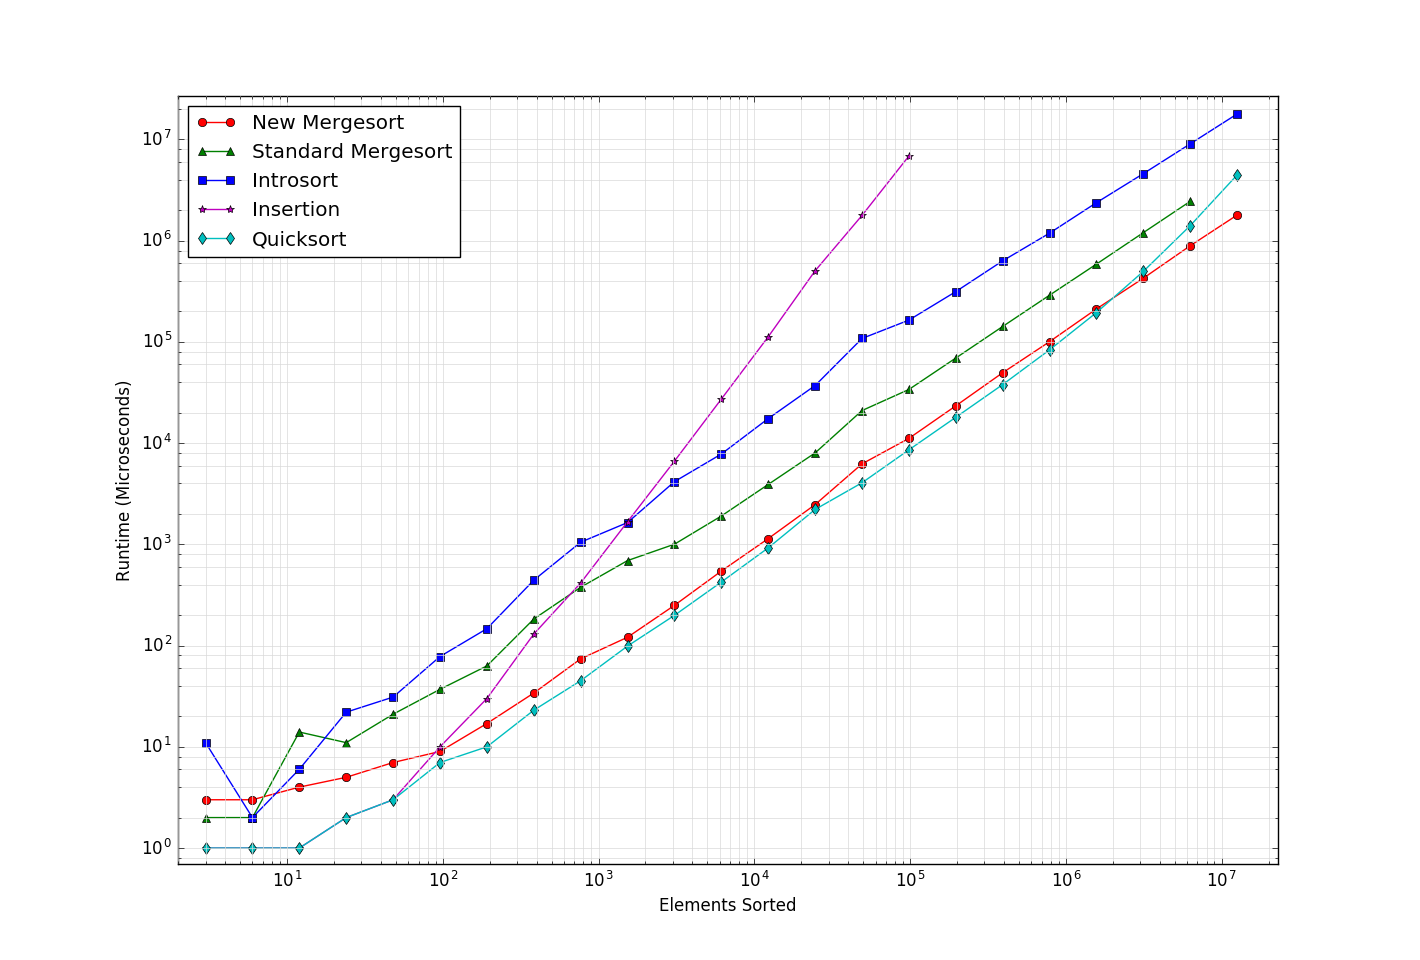
\includegraphics[width=6in]{figure_3.png}
		\caption{Algorithm Efficiency}
		\label{fig:algeff}
	\end{figure}
	
\section{Conclusion}

\pagebreak


\begin{thebibliography}{9}
	\bibitem{intro}
	Introduction to Algorithms, Third Edition,
	% todo: update author \emph{\LaTeX: a document preparation system},
	Addison Wesley, Massachusetts,
	2nd edition,
	1994.
	\bibitem{wiki}
	Wikipedia
	
\end{thebibliography}




\end{document}

